\documentclass{BeamerTemplate}

\title{Module 10 - Régression linéaire simple}

\graphicspath{{Images/Module 10/}}

\begin{document}
\begin{frame}[t]
  \titlepage
\end{frame}

%-------------------------------------------------------------------------------------------------------------------------------------





%%%%%%%%%%%%%%%%%%%%%%%%%%%%%%%%%%%
%%%%%%%%%%%%%%%%%%%%%%%%%%%%%%%%%%%
%%%%%%%%%%%%%%%%%%%%%%%%%%%%%%%%%%%

\section[Intro]{Introduction}

\subsection*{ }

\begin{frame}[t]
 \frametitle{Buts possibles d'une analyse de régression}

{\small
%Question fréquemment posée dans la plupart des domaines:

\alert{Quels effets les variables explicatives $X_1,\, X_2,\, X_3,\,... $ ont-elles sur la variable réponse $Y$?}

\begin{itemize}\itemsep2mm
\item Quels sont les effets de la météo, du jour de la semaine et du prix de l’essence sur le nombre de trajets effectués à vélo ?
\item Quel est l’impact de la vitesse du vent et de la hauteur des vagues sur les contraintes subies par une éolienne en mer?
\item Quel est l’impact de la distance à l’université, du moyen de transport utilisé et de l’horaire de cours sur le taux de présence en classe ?
\end{itemize}
}
\end{frame}

\begin{frame}[t]{Objectifs plus précis}

{\small
Étudier les relations entre des variables en se basant sur des données}.

\begin{itemize}

\item \alert{Prévision}: {\scriptsize {\it
\'Etant donné son âge, son poids, fumeur/non fumeur, combien
d'années un individu devrait-il survivre?}}

\item \alert{Sélection de variables}: {\scriptsize {\it
Parmi la température, l'ensoleillement, la pluie re\c{c}ue,
l'altitude, le trafic,  quelles variables ont une influence
significative sur l'orniérage des routes?}}

\item \alert{Spécification de modèle}: {\scriptsize {\it
Comment la durée de vie de transformateurs électriques varie-t-elle
en fonction de leur grosseur?}}

\item \alert{Estimation de paramètres}: {\scriptsize {\it
La luminosité en fonction de la distance des étoiles d'une certaine
galaxie est de la forme $L=K_1+K_2d+\sigma\varepsilon$, où $K_1$, $K_2$ et $\sigma$
sont des paramètres inconnus à être estimés à partir d'observations.}}
\end{itemize}

\end{frame}



%\subsection{Modèles de régression}

\begin{frame}[t]{Modélisation}

Exprimer la valeur de $Y$ \alert{en fonction} des valeurs de $X_1,\ldots,X_{k}$:
$${\color{green!70!black}{Y}}=\alert{f(}{\color{blue}{X_1,\ldots,X_{k}}}\alert{)}+\text{fluctuation aléatoire}
$$

\hspace{1cm}
\begin{tikzpicture}[thick]
\draw [green!70!black, ->  ] (6,9) -- (4,8);
\draw [blue, ->    ] (8.5,9) -- (9,8) ;
\end{tikzpicture}

\begin{tabular}{lll}
{\color{green!70!black}{variable réponse}} & & {\color{blue}{variables explicatives}}\\
{\color{green!70!black}{variable dépendante}} && {\color{blue}{variables indépendantes}}\\
{\color{green!70!black}{variable endogène}} & &{\color{blue}{variables exogènes}}\\
{\color{green!70!black}{issue}} && {\color{blue}{facteurs}}\\
{\color{green!70!black}{ }} & &{\color{blue}{covariables }}\\
{\color{green!70!black}{ }} & &{\color{blue}{``features'' }}\\
\end{tabular}

\end{frame}

\begin{frame}[t]{Apprentissage statistique/machine}

Estimer la fonction $f(~)$ dans un modèle du type
$${\color{green!70!black}{Y}}=\alert{f(}{\color{blue}{X_1,\ldots,X_{k}}}\alert{)}+\text{fluctuation aléatoire}
$$
à partir de $n$ observations (les informaticiens parlent ``d'exemples'')
$(Y_{1},X_{11},\dots,X_{1k}),\dots,(Y_{n},X_{n1},\dots,X_{nk})$
est ce que l'on appelle de \alert{l'apprentissage statistique} (apprentissage machine).
\end{frame}


\begin{frame}[t]{Exemple d'un modèle à une variable}
%Soit $Y$, la masse d'un homme de 30 ans en kg et\\ soit $X$, sa grandeur en cm. On a que
%$$Y=f(X)+\mbox{fluctuation aléatoire}$$

$${\color{green!70!black}{Y}}\quad =\quad \alert{f(}{\color{blue}{X}}\alert{)}\quad +\quad \text{fluctuation aléatoire}
$$

\hspace{1cm}
\begin{tikzpicture}[thick]
\draw [green!70!black, ->  ] (5.3,9) -- (3.5,8);
\draw [blue, ->    ] (7.5,9) -- (6.8,8) ;
\draw [black, ->    ] (10.6,9) -- (10.9,8) ;
\end{tikzpicture}

\begin{tabular}{p{2cm}p{3cm}p{5cm}}
{\color{green!70!black}{note finale d'un étudiant dans un certain cours}} & {\color{blue}{nombre d'heures d'étude de l'étudiant}}& deux étudiants peuvent avoir étudié le même nombre d'heures, mais avoir des notes différentes\\[2mm]
& {\color{blue}{(explique une partie de la note) }}& (partie de la note non expliquée par le temps d'étude)
\end{tabular}
\end{frame}


%\subsection{Régression linéaire}

\begin{frame}[t]{Modèle linéaire}
Un modèle de  régression \underline{linéaire}  représente $Y$ comme une \alert{fonction linéaire} des paramètres :
$$
Y=\beta_0+\beta_1X_1+\beta_2X_2+\cdots+\beta_{k}X_{k}+E,
$$
\begin{itemize}
\item[] \alert{$Y$}: variable réponse
\item[] \alert{$X_1,\ldots,X_{k}$}: variables explicatives
%\item[] \alert{$f_1,\ldots,f_{k}$}: transformations connues des variables explicatives
\item[] \alert{$\beta_0,\ldots,\beta_{k}$}: paramètres de valeur inconnue à estimer à l'aide d'observations.
\item[] \alert{$E$}: erreur aléatoire
\end{itemize}
\end{frame}

\section[Rég. lin. simple]{La régression linéaire simple}

\subsection[Modèle]{Le modèle et les postulats}

\begin{frame}[t]{Modèle de régression linéaire \underline{simple} (RLS)}

\alert{Une seule variable explicative $X$} qui explique une partie de la valeur de $Y$

\medskip
%Utile pour modéliser la relation entre $X$ et $Y$ lorsqu'un
$n$ paires d'observations indépendantes $(X_1,Y_1),\ldots,(X_n,Y_n)$, \alert{réparties autour d'une droite imaginaire}.\\

\vspace{5mm}


\begin{minipage}[b]{5cm}{
${\color{green!70!black}{Y_i}}\quad=\quad{\color{blue}{\beta_0+\beta_1X_i}}\quad+\quad E_i$\\ \hspace{2cm} $(i=1,\ldots,n)$

\vspace{0.5cm}
\underline{Postulats}:\\
\alert{$E_i\sim N(0,\sigma^2)$ indép.}

équivalent à

\alert{$Y_i|X_i\sim N(\beta_0+\beta_1X_i,\sigma^2)$ indép.}

\vspace{0.5cm}

}
\end{minipage}

\href{https://019fb41b-4471-cf03-efcd-4ed4b58271ba.share.connect.posit.cloud/}{Illustration}
\end{frame}

\begin{frame}[t]{À noter}
 Il est important de comprendre que nous obtenons des observations des paires de variables aléatoires $(X_1,Y_1),\dots,(X_n,Y_n)$. 
 Le modèle suppose que ces paires sont générées ainsi :
 \begin{itemize}
     \item<1-> $X_1,\dots,X_n$ sont soit des valeurs fixées, %(expérience planifiée, comme au
     %module précédent), 
     soit $n$ réalisations d'une variable aléatoire dont la loi
     ne nous intéresse habituellement pas.
     \item<2-> Sachant les $X_i$, les $Y_i$ sont des
     variables aléatoires normales indépendantes obtenues en ajoutant
     des erreurs $E_i$ i.i.d. $N(0,\sigma^2)$ à $\beta_0+\beta_1X_i$ :
     \alert{$~\Rightarrow Y_i=\beta_0+\beta_1X_i+E_i$ et, sachant $X_i$,
     on a $Y_i|X_i\sim N(\beta_0+\beta_1X_i,\sigma^2)$}.
 \end{itemize}

\uncover<2->{Dans ce cours, nous aurons que $\beta_0,\beta_1,\sigma^2$ sont des paramètres inconnus et $X_i$ est une valeur que l'on considère fixe %(pour la suite nous allons omettre le conditionnement sur
%$X_i$ pour alléger la notation)
.
}
\end{frame}

\begin{frame}[t]{Les postulats du modèle}

{\small
Conditions d'application à vérifier, en ordre d'importance, avant d'interpréter les intervalles de confiance et les tests d'hypothèses à venir:
\begin{itemize}\itemsep2mm
\item[P1] {\bf  linéarité:} l'espérance de $Y_i$ est linéaire par rapport à $X_i$;\\
    {\color{gray}{ $E(E_i)=0 \hspace{1cm} \Leftrightarrow \hspace{1cm} E(Y_i)=\beta_0+\beta_1X_i $ }}
\item[P2] {\bf homoscédasticité:}  la variance de $Y_i$ autour de la droite est homogène (elle ne dépend pas de $X_i$);\\
    {\color{gray}{$V(E_i)=\sigma^2 \hspace{1cm} \Leftrightarrow \hspace{1cm} V(Y_i)=\sigma^2$}}
\item[P3]  {\bf indépendance:}  les observations sont indépendantes;\\
    {\color{gray}{ $E_i$ indépendants \hspace{1cm} $\Leftrightarrow$ \hspace{1cm} $Y_i$ indépendants}}
\item[P4]  {\bf  normalité:} les $Y_i$ sont de loi normale autour de la droite.\\
    {\color{gray}{ $E_i\sim$ normale \hspace{1cm} $\Leftrightarrow$ \hspace{1cm} $Y_i\sim$
    normale}}
\end{itemize}
}
\end{frame}


\begin{frame}[t]{Éléments du modèle de RLS}
\centerline{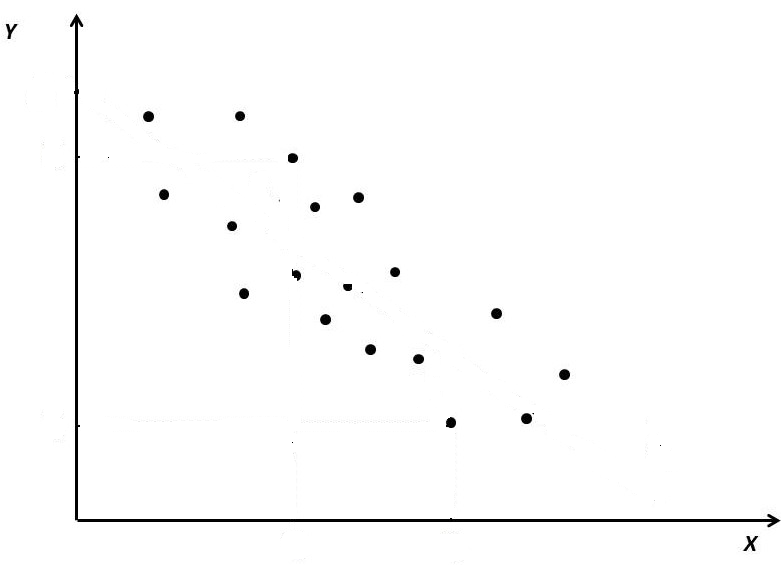
\includegraphics[height=6.5cm]{Images/Module 10/RLS1b-pts.png}}
\end{frame}

\begin{frame}[t]{Éléments du modèle de RLS}
\centerline{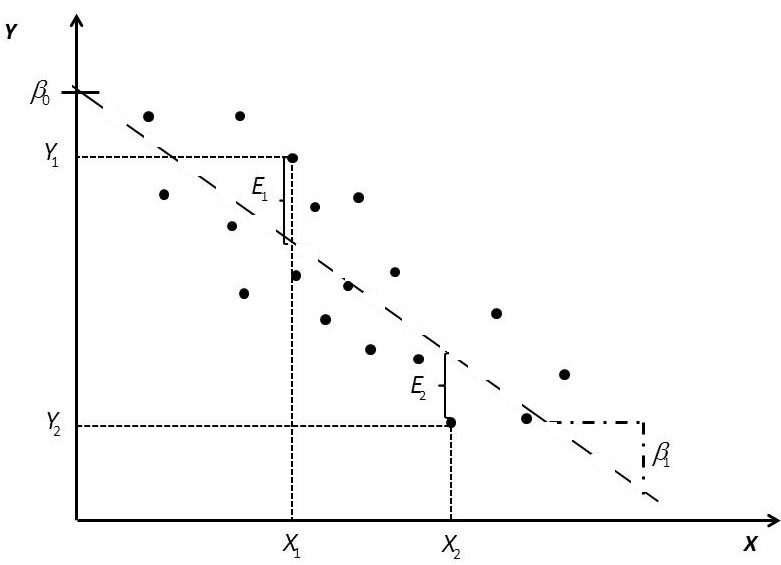
\includegraphics[height=6.5cm]{Images/Module 10/RLS1b-theo.png}}
\end{frame}


\begin{frame}[t]{Interprétation des paramètres $\beta_0$ et $\beta_1$}

Si le postulat de linéarité (P1) est vrai:
\begin{itemize}\itemsep2mm
\item<1-> {\color{blue}{$\beta_1$}}: \alert{Si on augmente $X$ d'une unité, alors la valeur moyenne de $Y$ augmente de $\beta_1$
unités}.\\
$\bullet$  $\beta_1>0$:  grands $X$  associés aux grands $Y$ et vice-versa (corrélation positive entre les variables). \\
$\bullet$  $\beta_1<0$:  petits  $X$ associés aux grands  $Y$.
\item<2-> {\color{blue}{$\beta_0$}}:  \alert{la valeur moyenne de $Y$ quand $X=0$}.\\
$\bullet$ Si la valeur $X=0$ est peu réaliste ou hors du domaine des données observées, $\beta_0$
  peut représenter une valeur peu significative ou aberrante.
  Néanmoins, le modèle de régression linéaire simple demeure pertinent pour les interprétations et prédictions lorsque $X$ est proche des valeurs effectivement observées.
\end{itemize}

\end{frame}

\begin{frame}[t]{Extrapolation dangereuse!}

{\small
%Soit $Y_i$ le rendement d'un procédé chimique et $X_i$ la concentration d'un certain catalyseur lors de la $i$-ème répétition d'une expérience, $i=1,\ldots,10$.
ATTENTION !!!! On \alert{ignore} la forme de la relation entre $X$ et $Y$ à l'extérieur de l'intervalle observé
pour les valeurs de $X_1,\dots,X_n$.
}

\centerline{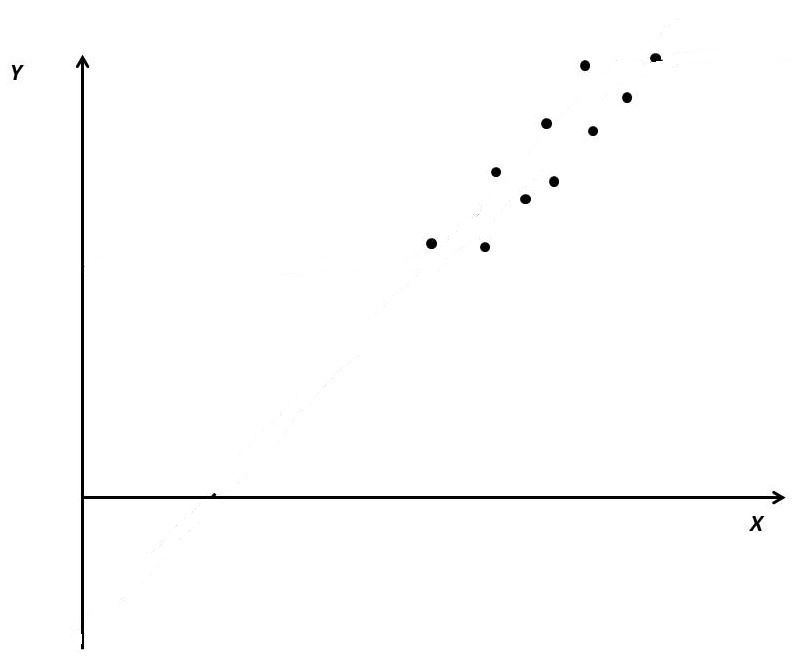
\includegraphics[height=5.25cm]{Images/Module 10/extrapol-vide.png}}
\end{frame}

\begin{frame}[t]{Extrapolation dangereuse!}

{\small
%Soit $Y_i$ le rendement d'un procédé chimique et $X_i$ la concentration d'un certain catalyseur lors de la $i$-ème répétition d'une expérience, $i=1,\ldots,10$.
ATTENTION !!!! On ignore la forme de la relation entre $X$ et $Y$ à l'extérieur de l'intervalle observé
pour les valeurs de $X_1,\dots,X_n$.
}

\centerline{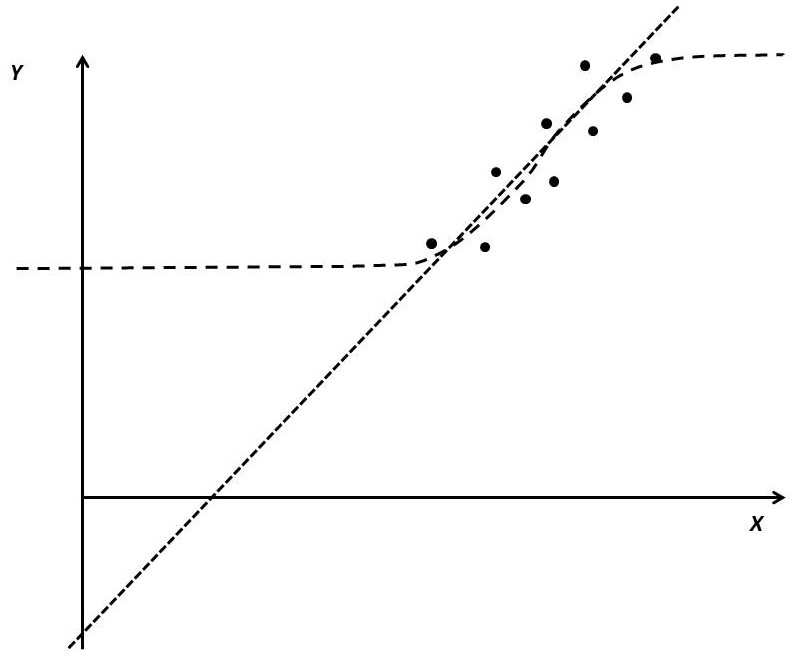
\includegraphics[height=5.25cm]{extrapol.jpg}}
\end{frame}


\subsection[Estimer $\beta_0$, $\beta_1$]{Estimation des paramètres $\beta_0$ et $\beta_1$}

\begin{frame}[t]{Estimation des paramètres  $\beta_0$ et $\beta_1$}

{\small
%En pratique, on observe $(X_1,Y_n),\ldots,(X_n,Y_n)$ mais on n'observe pas la vraie droite, c.-à-d.,
$\beta_0$ et $\beta_1$ : paramètres de valeurs inconnues.\\[1mm]
$\hat{\beta}_0$ et $\hat{\beta}_1$ : estimateurs des paramètres, obtenus en \alert{minimisant la partie inexpliquée de $Y$} (la fluctuation aléatoire):

\medskip


$$
SS_E\quad=\quad\sum_{i=1}^ne_i^2\quad=\quad\sum_{i=1}^n(Y_i-\hat{Y}_i)^2\quad=\quad\sum_{i=1}^n(Y_i-\hat{\beta}_0-\hat{\beta}_1X_i)^2,
$$
où

\begin{itemize}
\item[$\hat{Y}_i$]$=\hat{\beta}_0+\hat{\beta}_1X_i$ est la $i^e$ \alert{valeur ajustée}, ou \alert{valeur prédite} \\(la partie de $Y_i$ expliquée par le modèle ; hauteur de la ligne de régression
estimée en $x=X_i$)
\item[$e_i$]$=Y_i-\hat{Y}_i$ est le $i^e$ \alert{ résidu} \\(la partie de $Y_i$ inexpliquée par le modèle ; différence entre $Y_i$ et hauteur de la ligne estimée de régression en $x=X_i$).
\end{itemize}
}
\end{frame}







\begin{frame}[t]{Problème de minimisation}
En annulant les dérivées de $SS_E$ par rapport à $\hat\beta_0$ et $\hat\beta_1$, on obtient

% en résolvant les deux équations linéaires en $\hat{\beta}_0$ et $\hat{\beta}_1$ obtenues et en simplifiant (très bel exercice!!), on obtient
$$\begin{array}{|ll|}\hline &\\[-2mm]
%\begin{align*}
\hat{\beta}_1&%=\frac{\sum_{i=1}^n(X_i-\overline{X})Y_i}{\sum_{i=1}^n(X_i-\overline{X})^2}
=\dfrac{S_{XY}}{S_{XX}}\\[6mm]
\hat{\beta}_0&=\overline{Y}-\hat{\beta}_1\overline{X}\\[3mm]\hline
%\end{align*}
\end{array}$$

où\\

{\small
$S_{XX}=\sum\limits_{i=1}^n(X_i-\overline{X})^2\qquad = \qquad (n-1)\,s_X^2\quad = \quad\sum\limits_{i=1}^nX_i^2-n\overline{X}^2$

\bigskip
$S_{XY}=\sum\limits_{i=1}^n(X_i-\overline{X})(Y_i-\overline{Y})=\;\sum\limits_{i=1}^n(X_i-\overline{X})Y_i\;\;=\;\;
\sum\limits_{i=1}^nX_iY_i-n\overline{X}\overline{Y}.$
}
\end{frame}

\begin{frame}[t]{Éléments du modèle de RLS}
\centerline{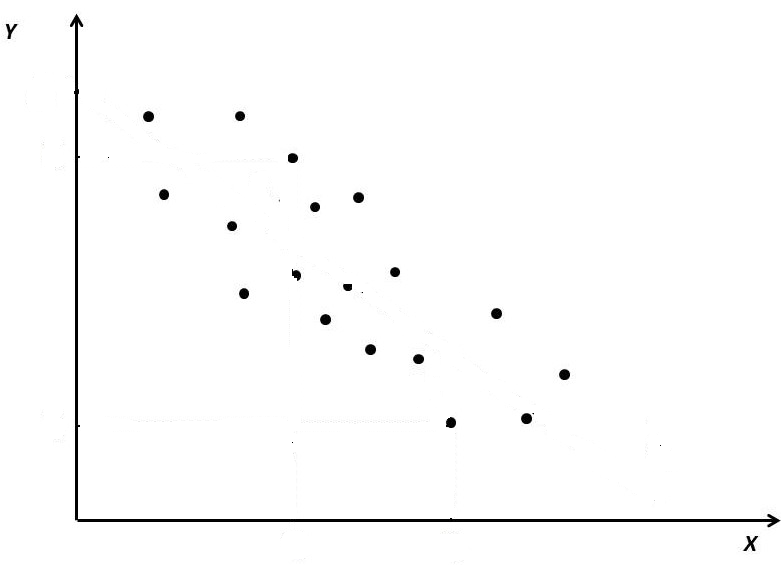
\includegraphics[height=6.5cm]{Images/Module 10/RLS1b-pts.png}}
\end{frame}

\begin{frame}[t]{Éléments du modèle de RLS}
\centerline{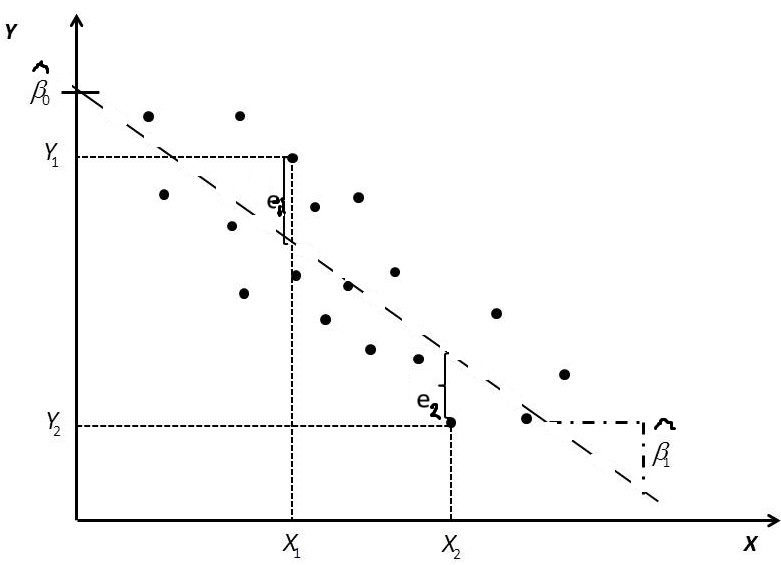
\includegraphics[height=6.5cm]{Images/Module 10/RLS1b-fit.png}}
\end{frame}



\begin{frame}[fragile]
\frametitle{Exemple 1: Absorption d'oxygène chez\\ 24 hommes qui courent 3,2 km}

\begin{minipage}[b]{4.5cm}
{\tiny
\begin{verbatim}
      VOLUME MAX.  TEMPS EN
SUJET   D'O2 (Y)  SECONDES (X)
   1       42.33      918
   2       53.10      805
   3       42.08      892
   4       50.06      962
   5       42.45      968
   6       42.46      907
   7       47.82      770
   8       49.92      743
   9       36.23     1045
  10       49.66      810
  11       41.49      927
  12       46.17      813
  13       48.18      858
  14       43.21      860
  15       51.81      760
  16       53.28      747
  17       53.29      743
  18       47.18      803
  19       56.91      683
  20       47.80      844
  21       48.65      755
  22       53.69      700
  23       60.62      748
  24       56.73      775
\end{verbatim}
}
\end{minipage}
\begin{minipage}[b]{6cm}{
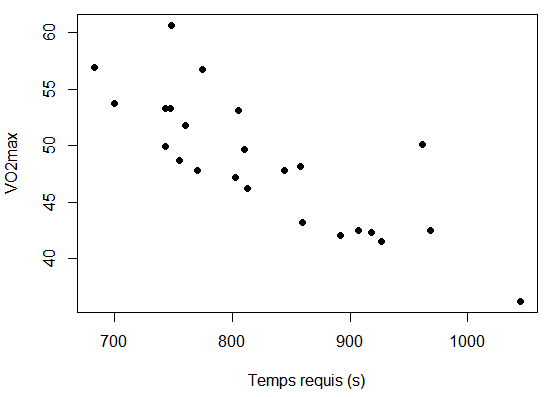
\includegraphics[width=8cm]{Ex9_4-R1.png}

}\end{minipage}
\end{frame}


\begin{frame}[t]{Exemple 1: Estimation des paramètres}

{\small %Avec {\it R Commander} ... ou à la main: on a que
On a effectué les calculs suivants:

\vspace{-0.7cm}
\begin{align*}
  \overline x = 826,5& &s_X^2 = 8593,8 & & \sum\limits_{i=1}^{24}x_iy_i=952\,885\\  
  \overline y = 48,55& &s_Y^2 = 34,1& & \\
\end{align*}

\vspace{-0.7cm}
Quelle est l'équation de la droite de régression estimée?}

$\hat\beta_1=\dfrac{S_{XY}}{S_{XX}}$

\vspace{7mm}

$\hat\beta_0=\overline{Y}-\hat{\beta}_1\overline{X}$

\vspace{7mm}

$\hat Y=\hat\beta_0+\hat\beta_1\,X$
\end{frame}


\begin{frame}[t]{ }

\centerline{\LARGE\bf \alert{QUIZ !}}
\bigskip

\begin{itemize}\itemsep1cm
\item Jacques a couru les 3,2 km en 10 secondes de plus que Marc, mais ils n'ont pas mesuré leur $VO_2max$. Quelle différence de $VO_2max$ le modèle ajusté prédit-il entre les deux hommes?
\item Vrai ou Faux: Il est raisonnable de dire que les hommes qui courent le 3,2 km en 0 seconde ont un $VO_2max$ moyen de 90,7.
\end{itemize}

\vspace{0.25cm}
\uncover<2->{
{\scriptsize
Pour votre curiosité : chatGPT nous informe que des $VO_2max$ de 90,7 ne sont pas complètement impossibles, mais absolument exceptionnels et n'ont été atteints que par quelques fondeurs ou cyclistes d'exception
(p.ex., on évalue celui de Pogacar à 89,4). 

Et un temps de 0 seconde est très
certainement plus que farfelu ! Jakob Ingebrigtsen détient la meilleure performance mondiale sur 2 miles ($\approx$ 3,218 km) avec un temps de 474 secondes ... son $VO_2max$ est estimé à 70-80.}
}
\end{frame}

\subsection[Tests $\beta_1=0$]{Tests d'hypothèses pour $H_0:\beta_1=0$}

\begin{frame}[t]{Relation non significative entre $Y$ et $X$}

%Si le postulat de linéarité est respecté, alors 
Une \alert{pente nulle pour la droite de régression ($\beta_1=0$) signifie qu'il n'y pas d'association entre les variables $Y$ et $X$}.
\medskip

$\Leftrightarrow$ La loi de $Y$ ne change pas avec la valeur de $X$ (la valeur espérée de $Y$ est égale à
$\beta_0$, peu importe la valeur de $X$.)

%En effet, dans ce cas on a que $E(Y|X)=\beta_0+\beta_1X=\beta_0+0X=\beta_0$, et donc

\begin{center}
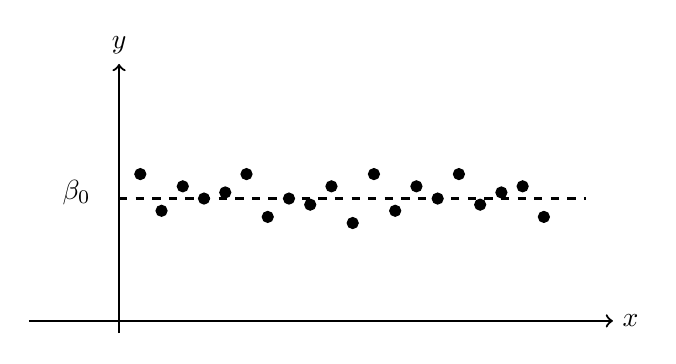
\begin{tikzpicture}
\begin{axis}[
    axis lines=middle,
    axis line style=thick,
    width=9cm,
    height=5cm,
    xtick=\empty,
    ytick=\empty,
    xlabel={$x$},
    ylabel={$y$},
    enlargelimits=0.05,
    ymin=0, ymax=2,
    xmin=-1.5, xmax=11,
    axis line style={->},
    xlabel style={right},
    ylabel style={above}
]

% Nuage de points centrés autour de y = 1
\addplot[
    only marks,
    mark=*,
    black
] coordinates {
  (0.5,1.2) (1,0.9) (1.5,1.1) (2,1.0) (2.5,1.05)
  (3,1.2) (3.5,0.85) (4,1.0) (4.5,0.95) (5,1.1)
  (5.5,0.8) (6,1.2) (6.5,0.9) (7,1.1) (7.5,1.0)
  (8,1.2) (8.5,0.95) (9,1.05) (9.5,1.1) (10,0.85)
};

% Ligne horizontale pointillée à y = 1
\addplot[dashed, thick] coordinates {(0,1) (11,1)};
\node at (axis cs:-1,1.05) {$\beta_0$};

\end{axis}
\end{tikzpicture}
\end{center}

\end{frame}

\begin{frame}[t]{Valeur de $\hat{\beta}_1$}

ATTENTION !!! Il faut résister à l'envie de dire que si
une valeur observée de $\hat{\beta}_1$ est ``près de zéro'',
on a une faible association entre $Y$ et $X$. 

P.ex. si on obtient $\hat{\beta}_1=2,35$
avec $X$ mesuré en mètres, si on refait exactement la même analyse avec
les mêmes données (donc association entre $Y$ et $X$ inchangée), mais avec $X$ mesuré en mm, on obtiendra $\hat{\beta}_1=0,00235$.

\medskip
La solution : Faire des inférences statistiques formelles (tests d'hypothèses, intervalles de confiance)
sur la valeur de $\beta_1$.
\end{frame}

\begin{frame}[t]{Tests sur la significativité de la relation linéaire}
Il existe deux approches équivalentes pour tester
$$
H_0:~\beta_1=0\text{\ \ \ \ vs\ \ \ \ }H_1:~\beta_1\neq0.
$$



\begin{Boite}{}{1) Analyse de la variance
 (Test $F$)}
 \end{Boite}



\begin{Boite}{}{2) Test $t$ sur $\beta_1$
 ou IC($\beta_1$)}
 \end{Boite}

\end{frame}

\begin{frame}[t]{1) Approche basée sur l'analyse de la variance}
On décompose la variabilité des $Y_1,\ldots,Y_n$ en deux sources:

$$\begin{array}{lccc}
\underbrace{\sum_{i=1}^n(Y_{i}-\overline{Y})^2}_{SS_T}=&
\underbrace{\sum_{i=1}^n(\hat{Y}_i-\overline{Y})^2}_{SS_{R}}&+&
\underbrace{\sum_{i=1}^n(Y_{i}-\hat{Y}_{i})^2}_{SS_E}\\[1cm]
\mbox{{\scriptsize Variabilité totale}} =&
\mbox{{\scriptsize Variabilité due au modèle}}& +&
\mbox{{\scriptsize Variabilité résiduelle}}.\\
 &
\mbox{{\scriptsize (variabilité expliquée par $X$)}}
\end{array}$$

%On a $n-1$ degrés de liberté pour $SS_T$, 1 degré de liberté pour $SS_R$ et $n-2$ degrés de liberté pour $SS_E$.
\end{frame}

\begin{frame}{Illustration de la décomposition de la variabilité}
\begin{center}
    

\begin{tikzpicture}
  \begin{axis}[
    axis lines=middle,
    xlabel={$x$},
    ylabel={$y$},
    xmin=0, xmax=11,
    ymin=0, ymax=11,
    xtick=\empty,
    ytick=\empty,
    width=12cm,
    height=8cm,
    enlargelimits=true,
    clip=true,
  ]

  % Données de points aléatoires autour de la droite y = 0.8x + 2
\addplot[
    only marks,
    mark=*,
    color=black
  ] coordinates {
   (1, 4.8)
    (2, 1.5)
    (3, 6.0)
    (4, 3.2)
    (5, 9.3)
    (6, 3.6)
    (7, 10.5)
    (8, 4.6)
    (9, 11.0)
  };


  % Droite de régression rose
  \addplot[
    domain=0:11,
    samples=2,
    thick,
    color=magenta,
  ] {0.8*x + 2};

  \end{axis}
\end{tikzpicture}
\end{center}
\end{frame}
\begin{frame}[t]{Trucs calculatoires}
%Très utiles pour résoudre des exercices "à la main":
\begin{align*}
SS_T&=\sum_{i=1}^n(Y_i-\overline{Y})^2\;=\;S_{YY}\;=\;(n-1)s^2_Y\;=\;\sum_{i=1}^nY_i^2-n\overline{Y}^2\\[4mm]
SS_R&=\sum_{i=1}^n(\hat{Y}_i-\overline{Y})^2=\hat{\beta}_1S_{XY}=\frac{(S_{XY})^2}{S_{XX}}
=\frac{\left(\sum\limits_{i=1}^nX_iY_i-n\overline{X}\,\overline{Y}\right)^2}{\sum\limits_{i=1}^nX^2_i-n\overline{X}^2}\\[5mm]
SS_E&=SS_T-SS_R
\end{align*}
\end{frame}

\begin{frame}[t]{Tableau d'analyse de la variance}

On résume  cette décomposition dans une table d'anova:


\begin{center}

{\renewcommand{\baselinestretch}{3}
{\scriptsize
\begin{tabular}{cccccc}\hline
Source de & Somme des & Degrés de & Carrés  & $F_0$ & Valeur $P$ \\[-4mm]
variabilité & carrés & liberté & moyens & & \\ \hline
Régression & $SS_{R}$ & $1$ & $MS_{R}=\dfrac{SS_R}{1}$ & $F_0=\dfrac{MS_{R}}{MS_E}$ & $P(F_{1,\,n-2}>F_0)$ \\
Erreur & $SS_E$ & $n-2$ & $MS_E=\dfrac{SS_E}{n-2}$ & & \\ \hline
Totale & $SS_T$ & $n-1$ & & & \\ \hline
\end{tabular}
}
    
}
\end{center}

\end{frame}

\begin{frame}[t]{Règle de décision du test}

{\small
\underline{Si $H_0: \beta_1=0$ est vraie} (pas d'association entre $X$ et $Y$):
 \begin{itemize}
 \item \alert{la majeure partie de la variabilité dans les $Y_i$ sera expliquée par la fluctuation aléatoire}
\item $SS_T\approx SS_E$ , et $MS_R$ prendra une petite valeur

%\alert{$\Rightarrow$ Une grande valeur de $SS_R/SS_T$ est donc de l'évidence contre $H_0$.}

\item $F_0=\dfrac{MS_R}{MS_E}=\dfrac{SS_{R}/1}{SS_E/(n-2)}\sim F_{1,\,n-2}$
\end{itemize}

\medskip
\underline{Si $H_1: \beta_1\ne0$ est vraie} (relation linéaire positive ou négative entre $X$ et $Y$):

 \begin{itemize}
 \item \alert{une bonne partie de la variabilité des $Y_i$ sera expliquée par $X$}
 \item $MS_R$ prendra une  valeur assez supérieure à $MS_E$ ($F_0$ sera grand)
\end{itemize}

{\color{blue}{Ainsi \underline{on rejette $H_0:\beta_1=0$} au seuil $\alpha$ lorsque $f_0>F_{\alpha;1,\,n-2}$.}}
}

\href{https://019fb41b-4471-cf03-efcd-4ed4b58271ba.share.connect.posit.cloud/}{Illustration}

\begin{frame}[t]{ }

\centerline{\LARGE\bf \alert{QUIZ !}}
\bigskip

Vrai ou faux?

\bigskip
\begin{itemize}\itemsep15mm
 \item Quand $H_0: \beta_1=0$ est vraie, les valeurs prédites de $Y$ sont ``proches'' de la moyenne $\overline y$.

\item Quand $H_0: \beta_1=0$ est vraie, l'estimation de la pente ($\hat\beta_1$) vaut exactement 0.
\end{itemize}


\end{frame}


\begin{frame}[t]{2) Approche basée sur la loi $t$}

{\small
On peut utiliser le fait que
\begin{align*}
\hat{\beta}_1&=\frac{S_{XY}}{S_{XX}}=\frac{\sum_{i=1}^n(X_i-\overline{X})Y_i}{\sum_{i=1}^n(X_i-\overline{X})^2}
=\sum_{i=1}^n\left[\frac{(X_i-\overline{X})}{\sum_{i=1}^n(X_i-\overline{X})^2}\right]Y_i
\end{align*}
est une combinaison linéaire des $Y_i\Rightarrow$
$$
\hat{\beta}_1\sim N\left(\beta_1,\frac{\sigma^2}{S_{XX}}\right)\Leftrightarrow
\frac{\hat{\beta}_1-\beta_1}{\sqrt{\frac{\sigma^2}{S_{XX}}}}\sim N(0,1)
$$
et ensuite
\alert{$$
\frac{\hat{\beta}_1-\beta_1}{\sqrt{\frac{MS_E}{S_{XX}}}}\sim t_{n-2}.
$$}

}
\end{frame}

\begin{frame}[t]{Règles de décision}
On peut facilement déduire les tests
d'hypothèses de niveau $\alpha$ suivants pour $H_0:~\beta_1=c$.
\medskip

Soit $T_0=\dfrac{\hat{\beta}_1-c}{\sqrt{MS_E/S_{XX}}}$.

\bigskip
$\begin{array}{llr}
H_1:&\beta_1\neq c\Rightarrow{\color{blue}{\text{rejeter $H_0$ si\ }|t_0|>t_{\alpha/2;n-2}}}& \\[5mm]
H_1:&\beta_1> c\Rightarrow\text{rejeter $H_0$ si\ }t_0>t_{\alpha;n-2}&\\[5mm]
H_1:&\beta_1< c\Rightarrow\text{rejeter $H_0$ si\ }t_0<-t_{\alpha;n-2}&
\end{array}$

\end{frame}

\begin{frame}[t]{Règles de décision}
Le cas qui nous intéressera le plus souvent $H_0:~\beta_1=0$.
\medskip

Donc $T_0=\dfrac{\hat{\beta}_1}{\sqrt{MS_E/S_{XX}}}$.

\bigskip
$\begin{array}{llr}
H_1:&\beta_1\neq 0\Rightarrow{\color{blue}{\text{rejeter $H_0$ si\ }|t_0|>t_{\alpha/2;n-2}}}& \alert{\text{équivalent à l'ANOVA}}\\[5mm]
H_1:&\beta_1> 0\Rightarrow\text{rejeter $H_0$ si\ }t_0>t_{\alpha;n-2}&\\[5mm]
H_1:&\beta_1< 0\Rightarrow\text{rejeter $H_0$ si\ }t_0<-t_{\alpha;n-2}&
\end{array}$

\end{frame}


\begin{frame}[t]{Exemple 2: significativité de la relation linéaire}

{\small
{\it R Commander} permet d'effectuer facilement le test $F$ et le test $t$ de
$$\begin{array}{l}H_0:~\beta_1=0\\H_1:~\beta_1\neq0\end{array}$$
 On peut aussi les faire ``à la main".

 \bigskip

\begin{minipage}{4cm}{
\begin{Boite}{ } 1)\underline{ANOVA}
\end{Boite}}
\end{minipage}

 \bigskip
 $SS_T=(n-1)s_y^2$

 \bigskip
 $SS_R=\dfrac{S_{XY}^2}{S_{XX}}$

 \bigskip
 $SS_E=SS_T-SS_R$


 }

\end{frame}
\begin{frame}[t]{Exemple 2}

{

\begin{tabular}{cccccc}\hline
Source de & Somme des & Degrés de & Carrés  & $F_0$ & Valeur $P$ \\
variabilité & carrés & liberté & moyens & & \\ \hline
& & &&&\\
Régression & $$ & $$ & $$ & $$ & $$ \\
& & &&&\\
Erreur & $$ & $$ & $$ & & \\ \hline
& & &&&\\
Totale & $$ & $$ & & & \\
& & &&&\\ \hline
\end{tabular}
}

\end{frame}


\begin{frame}[t]{Exemple 2}

\begin{minipage}{4cm}{
\begin{Boite}{ } 2) \underline{Test $t$}
\end{Boite}}
\end{minipage}
\vspace{3mm}

$H_0: \beta_1=0$\\
$H_1:\beta_1\ne 0$

\end{frame}
%%%%%%%%%%%%%%%%%%%%%%%%%%%%%%%%%%%
%%%%%%%%%%%%%%%%%%%%%%%%%%%%%%%%%%%
%%%%%%%%%%%%%%%%%%%%%%%%%%%%%%%%%%%

\section[Intervalles]{Intervalles de confiance et de prédiction}


\begin{frame}[t]{Estimateurs de $\beta_0$ et $\beta_1$}

\centerline{$Y_i=\beta_0+\beta_1X_i+E_i,\ \ \quad E_i\;\sim\;N(0,\sigma^2)$}

\bigskip

{\small
%Les vraies valeurs de $\beta_0$ et $\beta_1$ sont inconnues, et estimées en minimisant $SS_E$:

{\renewcommand{\arraystretch}{2}
$\begin{array}{c|c|c}
\text{Paramètre}&\text{Pente}&\text{Ordonnée à l'origine}\\\hline
\text{Estimateur}&\hat{\beta}_1%=\frac{\sum_{i=1}^n(X_i-\overline{X})Y_i}{\sum_{i=1}^n(X_i-\overline{X})^2}
=\dfrac{S_{XY}}{S_{XX}}%=\dfrac{\sum_{i=1}^n(X_i-\overline{X})Y_i}{\sum_{i=1}^n(X_i-\overline{X})^2}
&\hat{\beta}_0=\overline{Y}-\hat{\beta}_1\overline{X}\\\hline
\text{Espérance}&E(\hat{\beta}_1)=\beta_1&E(\hat{\beta}_0)=\beta_0\\\hline
\text{Variance}&V(\hat{\beta}_1)=\dfrac{\sigma^2}{S_{XX}}&V(\hat{\beta}_0)=\dfrac{\sigma^2}{n}+\dfrac{\sigma^2\,\overline X^2}{S_{XX}}\\[2mm]\hline
\text{Stat. inférence}& \dfrac{\hat{\beta}_1-\beta_1}{\sqrt{\dfrac{MS_E}{S_{XX}}}}\sim t_{n-2}& \dfrac{\hat{\beta}_0-\beta_0}{\sqrt{MS_E\left(\frac{1}{n}+\frac{\overline{X}^2}{S_{XX}}\right)}}\sim t_{n-2}
\end{array}$
}

%$S_{XX}=\sum_{i=1}^n(X_i-\overline{X})^2=\sum_{i=1}^nX_i^2-n\overline{X}^2$
%\bigskip
%$S_{XY}=\sum_{i=1}^n(X_i-\overline{X})(Y_i-\overline{Y})=\sum_{i=1}^n(X_i-\overline{X})Y_i= \sum_{i=1}^nX_iY_i-n\overline{X}\overline{Y}.$
}
\end{frame}
\subsection[IC $\beta_1$ et $\beta_0$]{Intervalles de confiance pour $\beta_1$ et $\beta_0$}

\begin{frame}[t]{Intervalle de confiance pour $\beta_1$}

On a que
$$P\left(-t_{\alpha/2;n-2}\le\frac{\hat{\beta}_1-\beta_1}{\sqrt{MS_E/S_{XX}}}\le t_{\alpha/2;n-2}\right)=1-\alpha.$$

En isolant $\beta_1$ au centre, on obtient l'intervalle de confiance de niveau $1-\alpha$  suivant pour
$\beta_1$:
{\color{blue}{$$
\hat{\beta}_1\pm t_{\alpha/2;n-2}\sqrt{\frac{MS_E}{S_{XX}}}.
$$}}
\end{frame}


\begin{frame}[t]{Intervalle de confiance pour $\beta_0$}

$\hat{\beta}_0$ est aussi une combinaison linéaire des $Y_i$, donc
$$
\frac{\hat{\beta}_0-\beta_0}{\sqrt{MS_E\left(\frac{1}{n}+\frac{\overline{X}^2}{S_{XX}}\right)}}\sim t_{n-2}.
$$

On obtient l'intervalle de confiance de niveau $1-\alpha$   pour
$\beta_0$:

{\color{blue}{$$
\hat{\beta}_0\pm t_{\alpha/2;n-2}\sqrt{MS_E\left(\frac{1}{n}+\frac{\overline{X}^2}{S_{XX}}\right)}.
$$}}
\end{frame}


\begin{frame}[t]{Exemple}
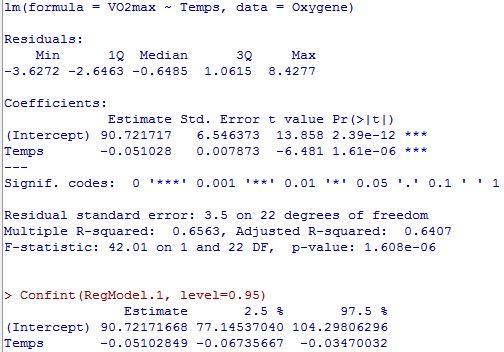
\includegraphics[scale = 0.75]{Images/Module 10/IC-VO2max.JPG}
\end{frame}



\subsection[IC($E(Y|x_0)$)]{Intervalle de confiance pour la valeur moyenne de $Y$ lorsque $X=x_0$}

\begin{frame}[t]{Estimation de $E(Y|X=x_0)$}

{\small
\begin{itemize}
\item<1-> Pour un \alert{$X$ fixé à $x_0$} , la valeur de $Y$ tourne autour de $\beta_0+\beta_1x_0$.
%\item<2-> On observera \alert{plusieurs} observations de $Y$
\item<2-> On veut faire de l'inférence sur \alert{la valeur moyenne de $Y$ à ce niveau $X=x_0$}, c'est-à-dire sur $E(Y|X=x_0)$.
%\item<4-> Sous les hypothèses du modèle de régression, cette valeur est $\beta_0+\beta_1x_0$.
\item<3-> Un estimateur sans biais de la vraie valeur moyenne $\beta_0+\beta_1x_0$ est
$$\hat{Y}_0=\hat{\beta}_0+\hat{\beta}_1x_0.$$
\end{itemize}
}
\end{frame}

\begin{frame}[t]{Intervalle de confiance pour la moyenne de $Y$ en $x_0$}
On peut montrer que
$$V(\hat{Y}_0)=V(\hat{\beta}_0+\hat{\beta}_1x_0)=\sigma^2\left[\dfrac1n+\dfrac{(x_0-\overline{X})^2}{S_{XX}}\right]$$
et que
$$
\frac{\hat{Y}_0-(\beta_0+\beta_1x_0)}{\sqrt{MS_E\left[\frac{1}{n}+\frac{(x_0-\overline{X})^2}{S_{XX}}\right]}}\sim t_{n-2}
$$
et donc un intervalle de confiance de niveau $1-\alpha$  pour $E(Y|X=x_0)$ est donné par

{\color{blue}{$$
\hat{Y}_0\pm t_{\alpha/2;n-2}\sqrt{MS_E\left[\frac{1}{n}+\frac{(x_0-\overline{X})^2}{S_{XX}}\right]}.
$$}}
\end{frame}

\subsection[IP($Y_0$)]{Intervalle de prédiction d'une valeur individuelle de $Y$ quand $X=x_0$}

\begin{frame}[t]{Une question un peu différente}
Au lieu d'estimer la valeur moyenne de $Y$ en $x_0$, supposons qu'on veut \alert{prédire la valeur \underline{d'une observation individuelle} de $Y$} pour un $X$ fixé.

\medskip
\uncover<2->{ Mathématiquement, %pour une valeur donnée $x_0$
on cherche à prédire la valeur de \alert{$\beta_0+\beta_1x_0+E_0$}.%, où $E_0$ est un terme d'erreur de loi $N(0,\sigma^2)$.

\medskip
L'estimateur ponctuel d'une observation individuelle est $$\hat{\beta}_0+\hat{\beta}_1x_0+0=\hat{\beta}_0+\hat{\beta}_1x_0$$
(le même que pour la valeur moyenne de $Y$... mais sa variance sera plus grande.)
}
\end{frame}

\begin{comment}
\begin{frame}[t]{La stratégie}
\begin{itemize}
\item<1-> $\hat{\beta}_0+\hat{\beta}_1x_0$ est un estimateur sans biais de $\beta_0+\beta_1x_0$
\item<2-> La meilleure fa\c{c}on d'estimer sans biais $E_i$ est de l'estimer par ... zéro
\item<3-> On a donc que l'estimateur ponctuel d'une observation individuelle est le même que pour la valeur moyenne de $Y$, soit $\hat{\beta}_0+\hat{\beta}_1x_0+0=\hat{\beta}_0+\hat{\beta}_1x_0$
\item<4-> On veut un intervalle de confiance pour $\beta_0+\beta_1x_0+E_0\Rightarrow$ ...
\end{itemize}
\end{frame}
\end{comment}

\begin{frame}[t]{Intervalle de prévision de $Y$ quand $X=x_0$}
On peut montrer que
$$\frac{\hat{Y}_0-(\beta_0+\beta_1x_0+E_0)}{\sqrt{MS_E\left[\frac{1}{n}+\frac{(x_0-\overline{X})^2}{S_{XX}}\right]+MS_E}}\sim t_{n-2},
$$
ce qui mène à l'intervalle de prévision pour $\beta_0+\beta_1x_0+E_0$
{\color{blue}{$$
\hat{Y}_0\pm t_{\alpha/2;n-2}\sqrt{MS_E\left[\alert{1+}\frac{1}{n}+\frac{(x_0-\overline{X})^2}{S_{XX}}\right]}.
$$}}
\end{frame}

\begin{frame}[t]{Exemple 3}

{\small

\begin{enumerate}[(i)]
\item Calculons une prévision ponctuelle et un intervalle de confiance à 95\% pour la valeur moyenne de l'absorption maximale d'oxygène ($VO_2max$) chez les hommes qui courent les 3,2 km en 15 minutes et 25 secondes;

\end{enumerate}}

\end{frame}
\begin{frame}[t]{Exemple 3}

{\small

\begin{enumerate}[(ii)]
\item Calculons une prévision ponctuelle et un intervalle de prévision à 95\% pour le $VO_2max$ d'un homme qui court 3,2 km en 15 min 25 s.

\end{enumerate}}


\end{frame}

\begin{frame}[t]{Exemple 3 (suite)}

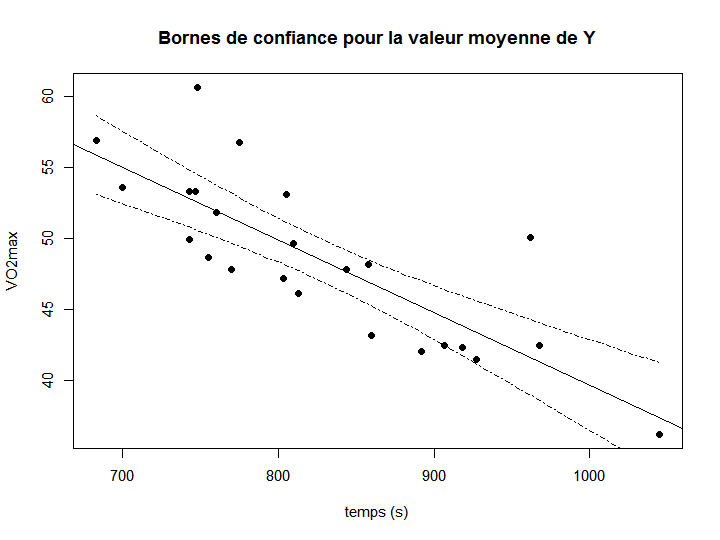
\includegraphics[width=10cm]{ICmoy.png}
\end{frame}

\begin{frame}[t]{Exemple  3 (suite)}

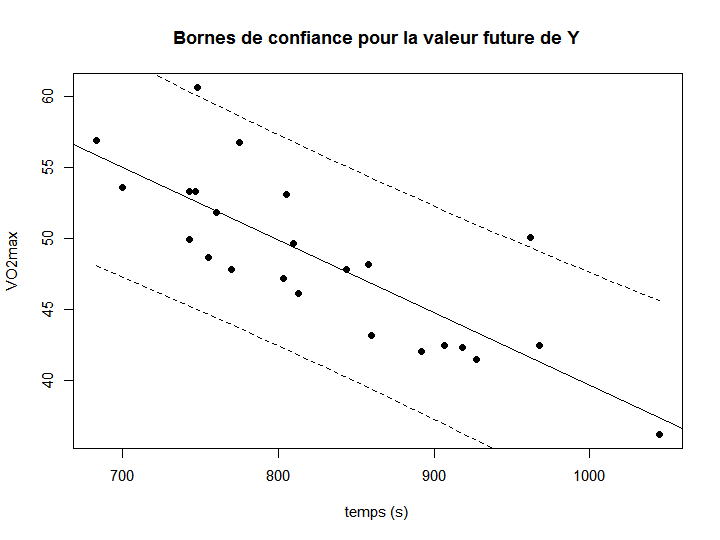
\includegraphics[width=10cm]{IPfutur.png}
\end{frame}




\section[Ajustement]{Corrélation et qualité de l'ajustement}

\begin{frame}[t]{Corrélation entre les valeurs de $Y$ et $X$}

Considérons à nouveau les $X_i$ comme des variables aléatoires.
Si nous retournons aux nuages de points
du module 4 sur les lois conjointes, on se doute qu'il devrait y avoir
un \alert{fort lien entre la valeur du coefficient
de régresison $\beta_1$ et la valeur
du coefficient de corrélation $\rho=corr(X,Y)$}.

\vspace{1cm}

\href{https://019fb41b-ce0f-240d-6ec5-496610d992e9.share.connect.posit.cloud/}{Illustration}
\end{frame}


\begin{frame}[t]{Estimation  de $\rho$}

{\small
On peut montrer que 
$$\rho=\frac{\beta_1\sigma_X}{\sqrt{\beta_1^2\sigma_X^2+\sigma^2}}=
\beta_1\dfrac{\sigma_X}{\sigma_Y}.$$ 
  

%On voit bien le lien  entre les estimations de $\beta_1$ et  de $\rho$.

$\rho$ est estimé par le coefficient de corrélation échantillonnal $r$ :}
{\footnotesize
$$\hat\rho=\alert{r=\hat\beta_1\dfrac{s_X}{s_Y}}=\frac{S_{XY}}{\sqrt{S_{XX}S_{YY}}}=\frac{\sum\limits_{i=1}^n(X_i-\overline{X})(Y_i-\overline{Y})}
{\sqrt{\sum\limits_{i=1}^n(X_i-\overline{X})^2\sum\limits_{i=1}^n(Y_i-\overline{Y})^2}}
.$$}

{\small
\begin{tabular}{ccc}
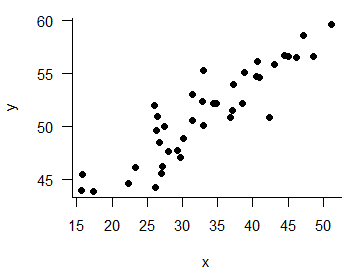
\includegraphics[width=3cm]{rho9.png}&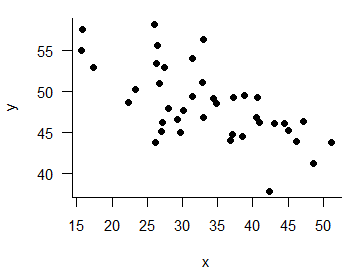
\includegraphics[width=3cm]{rho6.png}&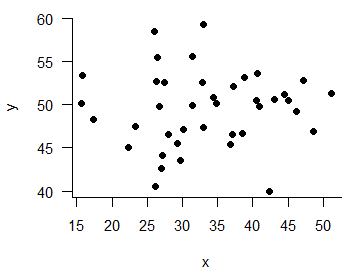
\includegraphics[width=3cm]{rho1.png}\\
 $\rho_{\text{simulé}}=0,9$ & $-0,6$ &$ 0,1$\\
$r =0,90$ & $-0,640$ & $0,041$\\
$R^2= 0,809$ &$0,409$&$ 0,0017$
\end{tabular}
}

\end{frame}
\begin{comment}
\medskip
\uncover<2->{
Comme on avait $\hat{\beta}_1=S_{XY}/S_{XX}$, on remarque
$$\hat{\beta}_1=r\sqrt{\frac{S_{YY}}{S_{XX}}}=r\,\dfrac{s_Y}{s_X}\quad\Leftrightarrow\quad
r=\hat{\beta}_1\sqrt{\frac{S_{XX}}{S_{YY}}}.$$}
}


set.seed(14)
sx<-10
sy<-5
p<-0.9
x<-rnorm(40,mean=30, sd=sx)
y<-rnorm(40,mean=50+p*sy*(x-30)/sx,sd=sy*sqrt(1-p^2))
cor(x,y)

png("rho9.png",width=4,height=3,unit="in",res=90)
par(mar=c(4,4,1,1))
plot(x,y,pch=19,las=1,bty="l")
dev.off()
\end{comment}


\subsection{Coefficient de détermination $R^2$}

\begin{frame}[t]{Le coefficient de détermination $R^2$}

Est-ce que $X$ "explique  bien" $Y$?

\medskip
Le \underline{coefficient de détermination} ($R^2$), soit \alert{la proportion de
la variabilité dans les $Y_i$ qui est expliquée par le modèle de régression} (donc par $X$), est une quantité très utilisée pour juger de la qualité d'un modèle de régression linéaire.

\begin{align*}
R^2&=\frac{SS_R}{SS_T}\\
&{\color{gray}{=\frac{S^2_{XY}/S_{XX}}{S_{YY}}=\frac{S_{XY}}{S_{XX}}\frac{S_{XY}}{S_{YY}}}}\\
&{\color{gray}{=\hat{\beta}_1\frac{S_{XY}}{S_{YY}}=\hat{\beta}_1^2\frac{S_{XX}}{S_{YY}}}}\\
&=r^2.
\end{align*}

\end{frame}


\begin{frame}[t]{Exemple 4 sur le $VO_2max$}
%$\Rightarrow$ \alert{Plus la corrélation entre $X$ et $Y$ est forte, plus grande sera la proportion de la variabilité dans la valeur des $Y_i$ expliquée par le modèle de régression}.

Coefficient de détermination :

\vspace{3cm}

Coefficient de corrélation échantillonnal :
\end{frame}


\section[Valider postulats]{Validation du modèle: Analyse des résidus}

\begin{frame}[t]{Une question avant de débuter}
Si on reprend l'exemple de la résistance du tissu du module 9, aurait-on pu utiliser la régression linéaire pour répondre à la question posée?
    \begin{center}
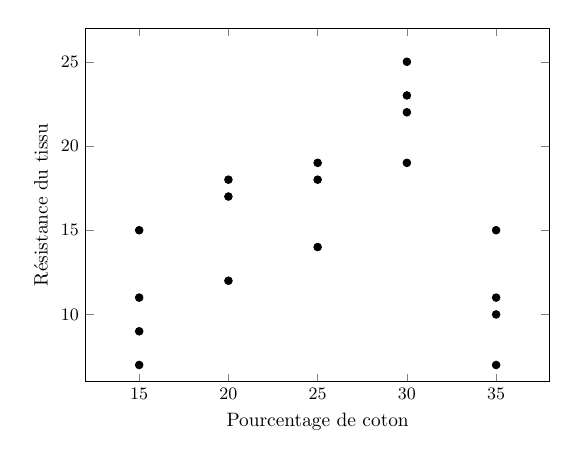
\begin{tikzpicture}[scale = 0.7]
  \begin{axis}[
    xlabel={Pourcentage de coton},
    ylabel={Résistance du tissu},
    xmin=12, xmax=38,
    ymin=6, ymax=27,
    width=10cm,
    height=8cm,
    only marks,
    mark=*,
    tick label style={font=\small},
    grid=none
  ]

  % Points extraits du graphique
  \addplot[color=black, mark=*] coordinates {
    (15,7) (15,15) (15, 11) (15, 9)
    (20,12) (20,17) (20,18)
    (25,14) (25,18) (25,19)
    (30, 19) (30,22) (30,23) (30,25)
    (35,7) (35,10) (35,11) (35, 15)
  };

  \end{axis}
\end{tikzpicture}
\end{center}
\end{frame}

\begin{frame}[t]{Validation du modèle: Analyse des résidus}
La validité des conclusions de l'analyse statistique du modèle de régression
dépend du respect des postulats (P1) à (P4).

\small
\begin{itemize}
\item[P1] {\bf  linéarité:} l'espérance de $Y_i$ est linéaire en $X_i$;
\item[P2] {\bf homoscédasticité:} $V(E_i)=V(Y_i)=\sigma^2$  (ne dépend pas de $X_i$);
\item[P3]  {\bf indépendance:} $E_1,\ldots,E_n$ indépendants (idem pour $Y_i$);
\item[P4]  {\bf  normalité:} $E_i\sim$ loi normale autour de la droite.
\end{itemize}
\normalsize

\medskip
Comme ces \alert{postulats portent tous sur le comportement aléatoire des termes d'erreur $E_i$}, nous les vérifierons à l'aide des résidus
$$
e_i=Y_i-(\hat{\beta}_0+\hat{\beta}_1X_i)=Y_i-\hat{Y}_i.
$$
\end{frame}


\subsection{(P1) Linéarité}

\begin{frame}[t]{(P1) Linéarité: Validation graphique}


\begin{itemize}
\item \alert{Un graphique de dispersion des paires $(x_i,y_i)$}: devrait montrer un nuage de points distribués de fa\c{c}on symétrique autour d'une ligne droite.
\item \alert{Un graphique des paires $(\hat{Y}_i,e_i)$}: devrait montrer un nuage de points distribués symétriquement autour de l'axe des abscisses.
\end{itemize}
\end{frame}

\begin{frame}[t]{Exemples de nuages de points}

\vspace*{-3mm}

{\small
\begin{tabular}{cc}
Linéarité raisonnable&Linéarité raisonnable\\
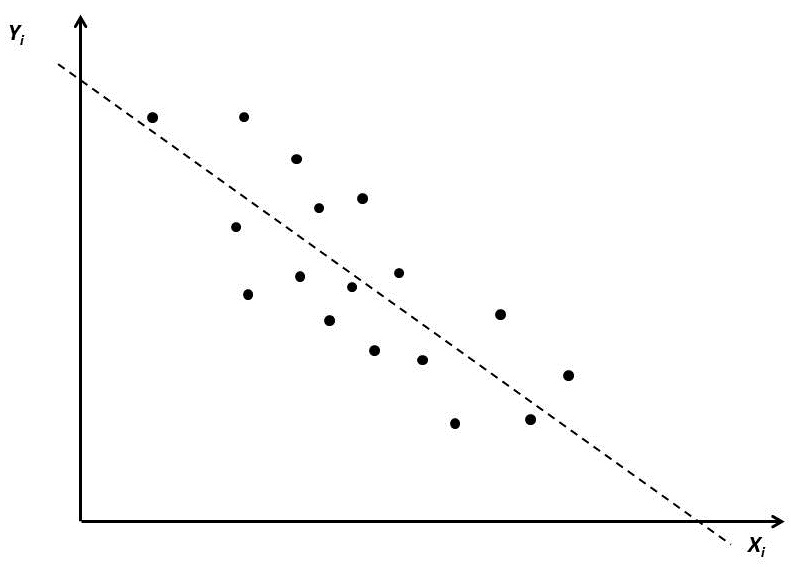
\includegraphics[width=1.8in]{yixiOK2.jpg} &
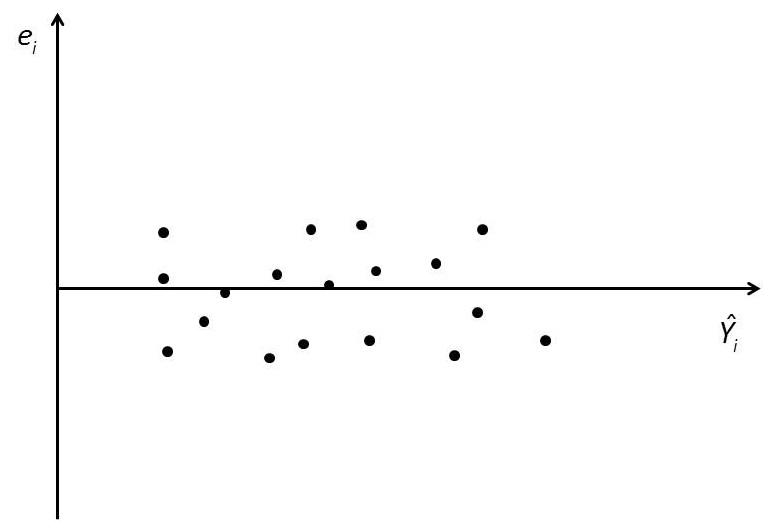
\includegraphics[width=1.8in]{eiyiOK2.jpg} \\
Linéarité déraisonnable&Linéarité déraisonnable\\
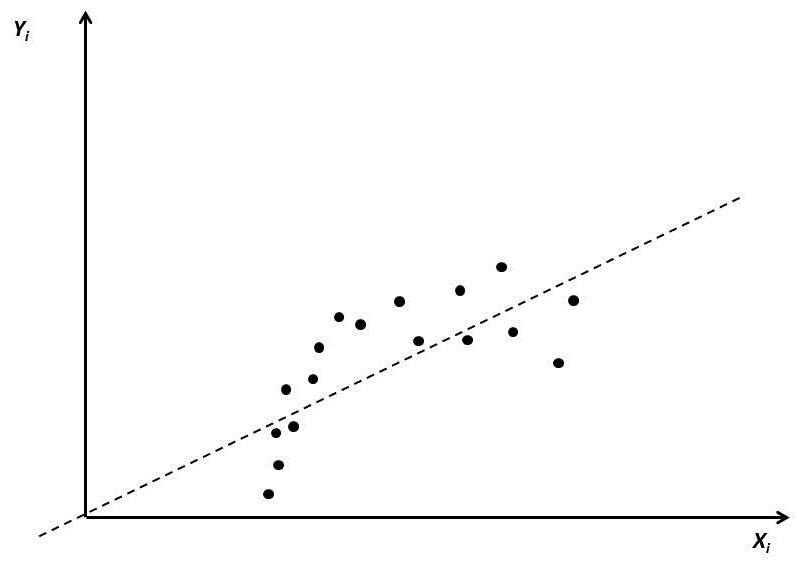
\includegraphics[width=1.8in]{yixiNOTOK2.jpg} &
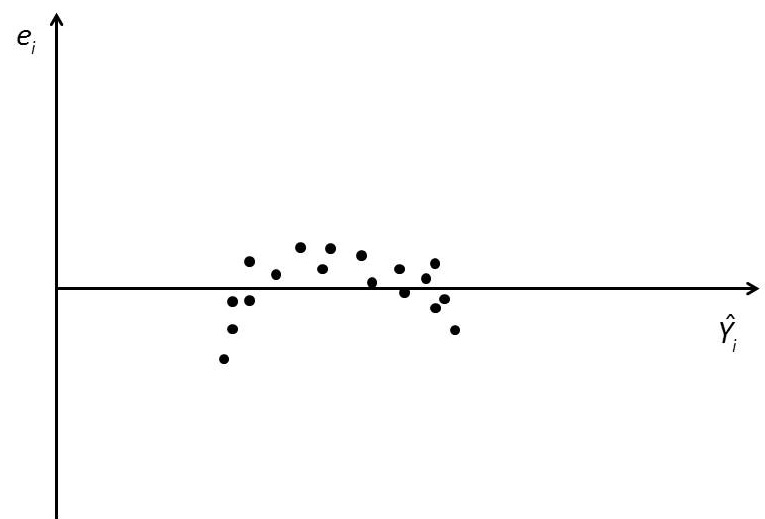
\includegraphics[width=1.8in]{eiyiNOTOK2.jpg} \\
\end{tabular}
}
\end{frame}

\subsection{(P2) Homoscédasticité (homogénéité de la variance)}

\begin{frame}[t]{(P2) Homoscédasticité}
\begin{itemize}
\item \alert{Un graphique des $e_i$ en fonction des $\hat{Y}_i$}: devrait montrer que la variabilité des $e_i$ demeure constante pour toute valeur de $\hat{Y}_i$.
\end{itemize}
\end{frame}

\begin{frame}[t]{Exemples de nuages de points}

\vspace*{-3mm}

{\small
\begin{tabular}{cc}
Homoscédasticité raisonnable&\\
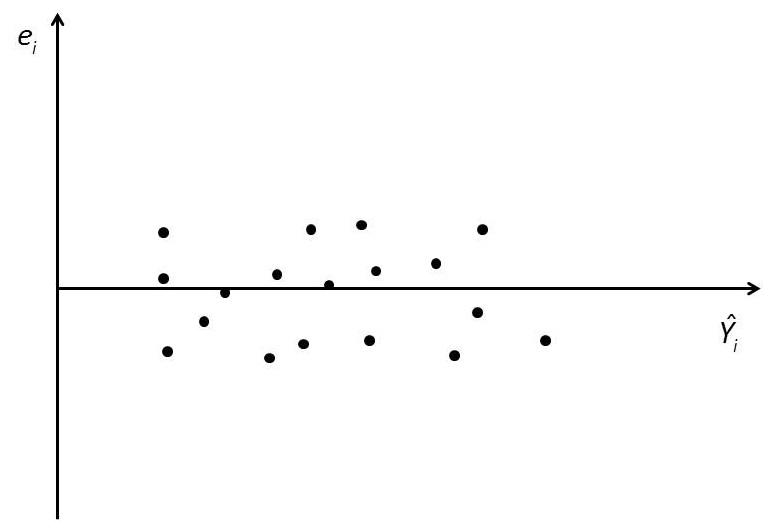
\includegraphics[width=1.8in]{eiyiOK2.jpg} &\\
Homoscédasticité déraisonnable&Homoscédasticité déraisonnable\\
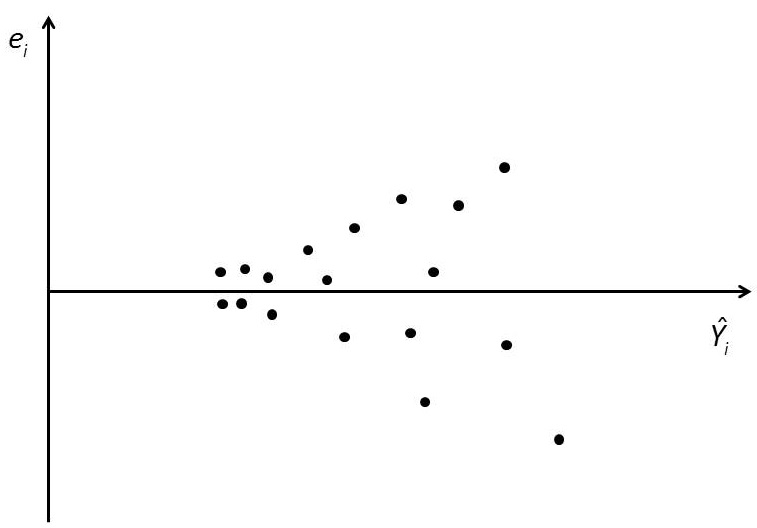
\includegraphics[width=1.8in]{hetero1-2.jpg} &
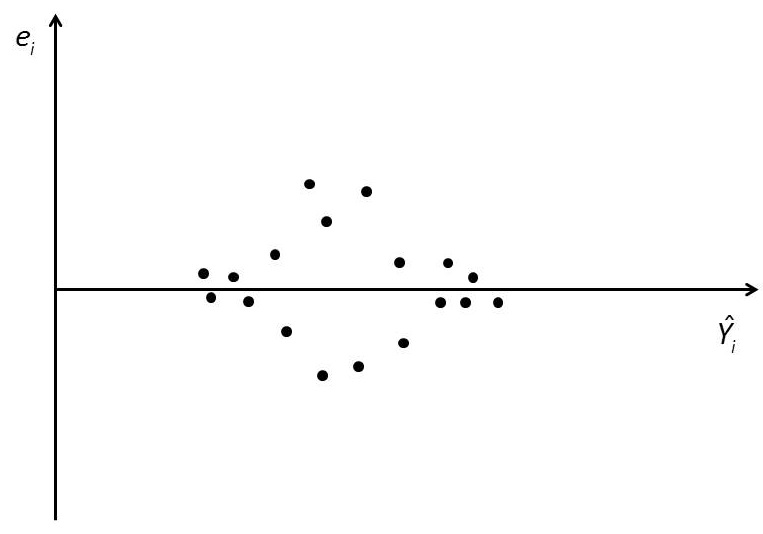
\includegraphics[width=1.8in]{hetero2-2.jpg} \\
\end{tabular}
}
\end{frame}



\subsection{(P3) Indépendance}

\begin{frame}[t]{(P3) Indépendance: Difficile à vérifier!}

{\small
C'est la collecte des données qui en est garante. Il faut s'assurer qu'\alert{aucune variable à part $X_i$ n'ait pu avoir une influence sur les valeurs observées}.

\medskip
Exemple d'une mauvaise collecte:
\begin{itemize} \item les observations 1, 2, 3, 4 sont prises par l'employé A qui a tendance à surestimer $Y$;
\item les mesures 5, 6, 7 et 8 sont prises par l'employé B qui a tendance à sous-estimer $Y$;
\item Problème: les observations prises par un même employé seront corrélées.
\end{itemize}
}
\end{frame}

\begin{frame}[t]{Données chronologiques}

{\small
Il peut aussi y avoir de la corrélation lorsque les observations sont prises de fa\c{c}on trop rapprochées dans le temps (ou l'espace).\\
Si les valeurs de $i=1,\ldots,n$ correspondent à un \underline{ordre chronologique}, le \alert{graphique des $e_i$ en fonction de $i$ } pourrait révéler un problème de corrélation positive entre les résidus rapprochés (``effet de grappe'').
}

\begin{center}
\begin{tabular}{cc}
Pas d'effet chronologique & Effet de grappe\\
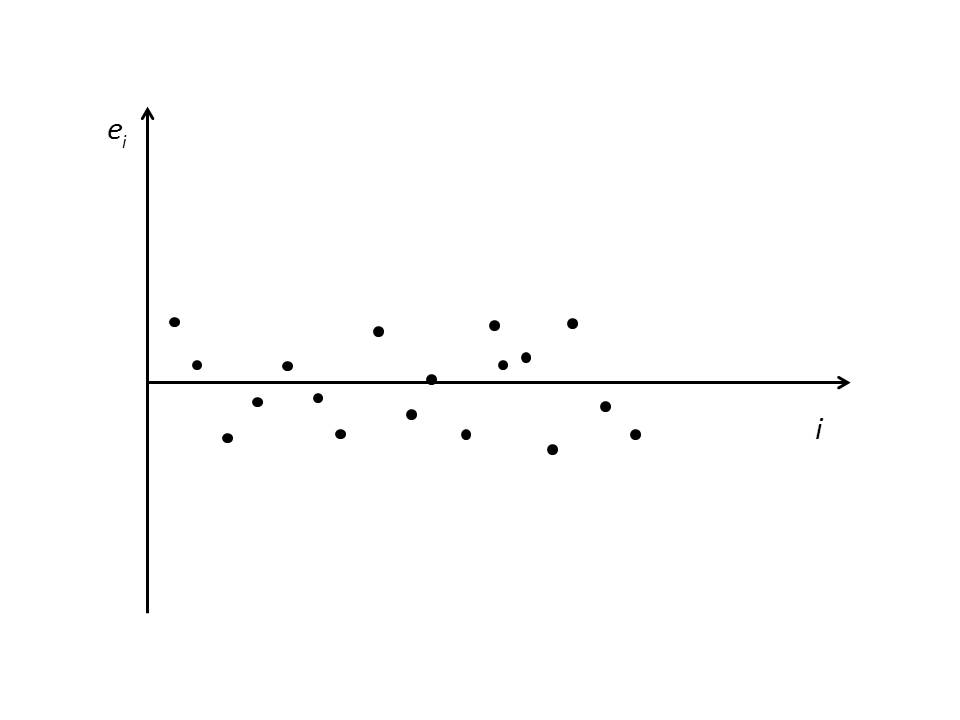
\includegraphics[width=2.17in]{eiiOK.jpg} &
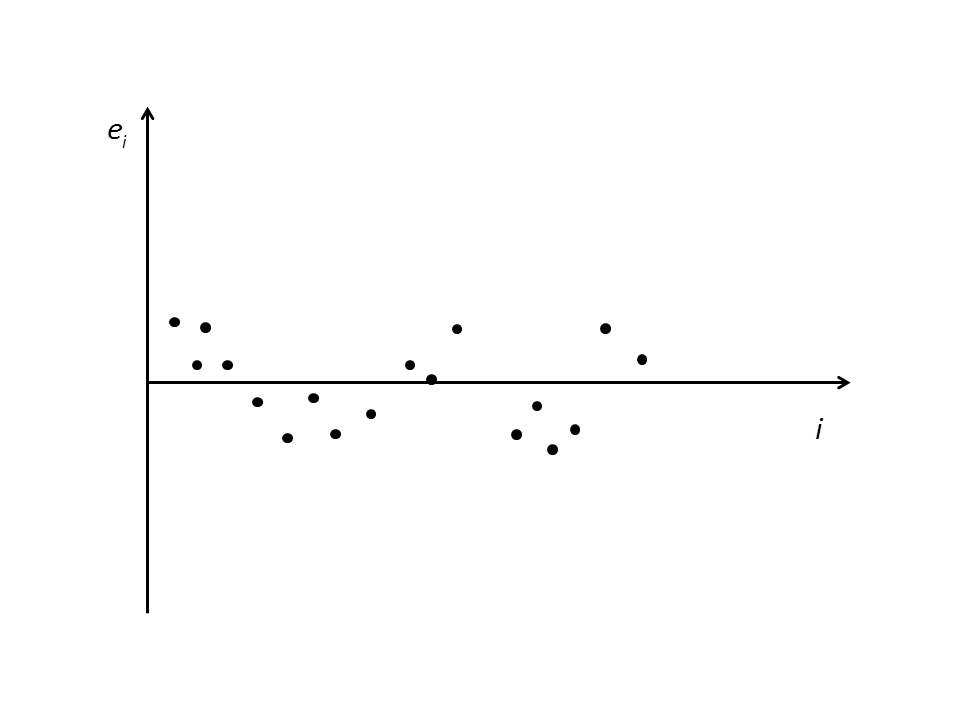
\includegraphics[width=2.17in]{eiiNOTOK.jpg} \\
\end{tabular}
\end{center}
\end{frame}


\subsection{(P4) Normalité}

\begin{frame}[t]{(P4) Normalité}
\begin{itemize}
\item \alert{histogramme des résidus}
\item \alert{graphique quantile-quantile normal des résidus }
\item \alert{diagramme en boîte des résidus}
\end{itemize}
\end{frame}

\begin{frame}[t]{Exemple 5 sur l'absorption d'oxygène}
% Des graphiques permettant de valider les postulats d'homoscédasticité et de normalité pour l'exemple sur l'absorption de l'oxygène suggèrent que l'hypothèse d'homoscédasticité semble raisonnable, mais on peut mettre en doute la normalité ...
\vspace*{-3mm}

\begin{tabular}{ll}
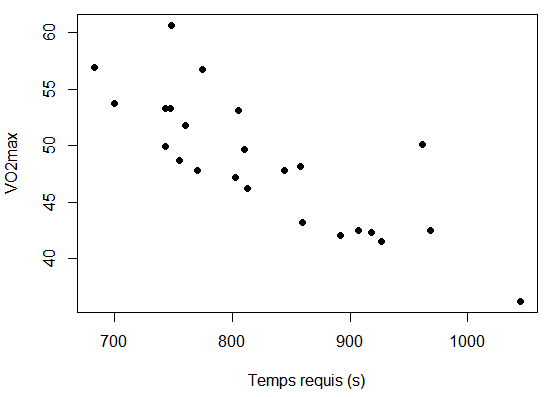
\includegraphics[width=1.8in]{Ex9_4-R1.png} &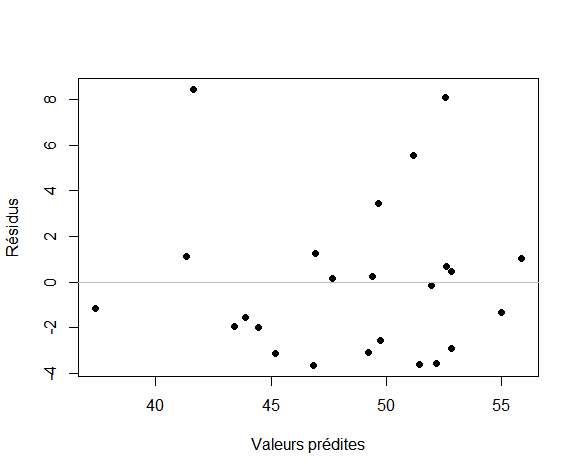
\includegraphics[width=1.8in]{Ex9_7-R1.png}\\
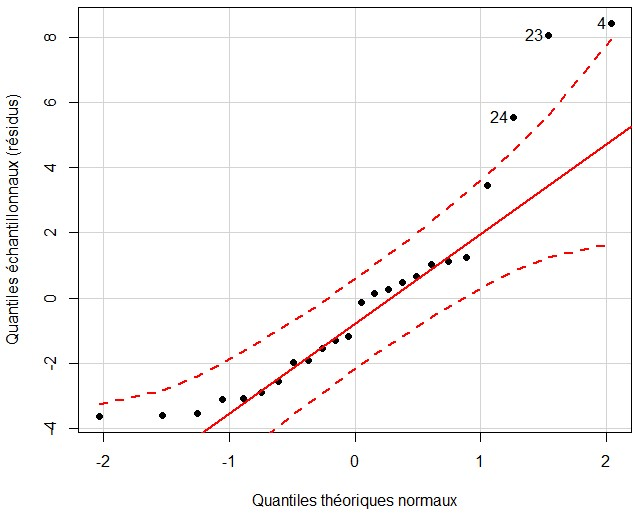
\includegraphics[width=1.8in]{Ex9_7-R3.jpg} & 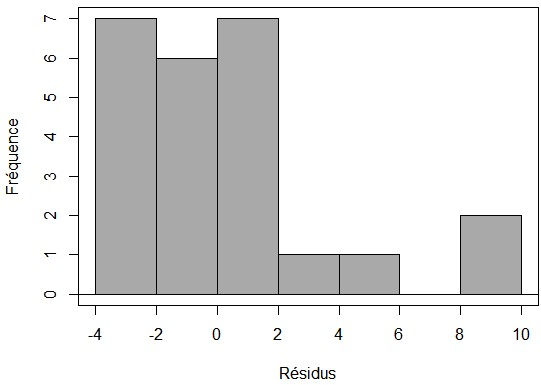
\includegraphics[width=1.8in]{Ex9_7-R2.jpg}
\end{tabular}
\end{frame}

\subsection{Solution aux problèmes: transformer $X$ et/ou $Y$}\label{sec:transfo}

\begin{frame}[t]{Que faire si les postulats ne sont pas respectés?}

{\small
Lorsque les postulats de linéarité, d'homoscédasticité ou de normalité ne sont pas respectés, on tente de  \alert{ transformer $Y$ ou $X$} pour régler le problème.
\begin{itemize}
\item<2-> \underline{Problème de non-linéarité}: on peut s'inspirer de la forme du nuage de points pour trouver une relation plus représentative de la tendance. Par exemple:
    \begin{itemize}\itemsep2mm
    \item<2-> $X_i^*=X_i^2\quad\;\Rightarrow\quad Y_i=\beta_0+\beta_1\,\alert{X_i^2}+E_i$
    \item<2-> $X_i^*=\text{ln}(X_i)\quad\Rightarrow\; Y_i=\beta_0+\beta_1\,\alert{\text{ln}(X_i)}+E_i$
    \item<2-> $X_i^*=1/X_i\quad\Rightarrow\quad Y_i=\beta_0+\beta_1\,\alert{[1/X_i]}+E_i$
    \item<3-> $Y_i^*=\sqrt{Y_i}\quad\Rightarrow\quad \alert{\sqrt{Y_i}}=\beta_0+\beta_1\,X_i+E_i$
    \item<3-> $Y_i^*=\text{ln}(Y_i)\quad\Rightarrow\quad \alert{\text{ln}(Y_i)}=\beta_0+\beta_1\,X_i+E_i$
    \end{itemize}
%\item<3-> D'autres transformations fréquentes sont $X_i^*=\ln X_i$, $X_i^*=1/X_i$ ou $X_i^*=\sqrt{X_i}$.
%\item<4-> De la même fa\c{c}on, on peut remplacer $Y_i$ par une transformation $Y^*_i$ dans le modèle pour régler un problème de linéarité.
\item<4-> Parfois, il faut transformer et \alert{$X$ et $Y$} pour parvenir à une relation linéaire. On peut aussi ajuster un modèle polynomial avec les outils de la régression multiple.
\end{itemize}
}
\end{frame}

\begin{frame}[t]{Que faire si les postulats ne sont pas respectés?}

{\small
\begin{itemize}
\item \underline{Problème d'hétéroscédasticité ou de non-normalité}: un changement dans l'échelle de $Y$ créé par \alert{une transformation de $Y$} pourra parfois stabiliser la variance ou améliorer la normalité. Par exemple:
    \begin{itemize}\itemsep2mm
    \item $Y_i^*=\sqrt{Y_i}\quad\Rightarrow\quad \alert{\sqrt{Y_i}}=\beta_0+\beta_1\,X_i+E_i$
    \item $Y_i^*=\text{ln}(Y_i)\;\Rightarrow\quad \alert{\text{ln}(Y_i)}=\beta_0+\beta_1\,X_i+E_i$
    \item $Y_i^*=1/Y_i\quad\Rightarrow\quad \alert{1/Y_i}=\beta_0+\beta_1\,X_i+E_i$
    \end{itemize}
\item  \underline{Problème de dépendance entre les observations}: refaire l'échantillonnage (!) ou utiliser des modèles statistiques qui prennent en compte des structures de dépendance entre les données (non couverts dans ce cours).
\end{itemize}
}
\end{frame}


\begin{frame}[t]{Réponses aux exemples}

{\scriptsize

\begin{enumerate}\itemsep 1mm
  \item  $\hat Y = 90,7 - 0,051 X$
  \item {\scriptsize
\begin{enumerate}[(i)]\itemsep 1mm
        \item  Anova: Valeur P = $P(F_{1,22}>42)\approx 0$. On rejette $H_0\beta_1=0$, le lien linéaire est significatif.
        \item Test $t$: Puisque $|t_{obs}|=|-6,48| > t_{0,025;22}=2,024$, on rejette $H_0$ (même valeur P et conclusion que test $F$).
        \end{enumerate}}
  \item \begin{enumerate}[(i)]\itemsep 1mm
        \item $ 43,5\pm 2,19$
        \item $ 43,5\pm 7,58$
        \end{enumerate}
  \item $R^2=0,6563,\; r=-0,81$
 \item linéarité du lien et homoscédasticité respectées, normalité des erreurs problématique
  \end{enumerate}

 }
\end{frame}
\end{document}